\section{Результати}

А цій задачі константа Ліпшиця мені невідома, тому тут наводяться результати лише адаптивних алгоритмів.

\begin{figure}[H]
    \centering
    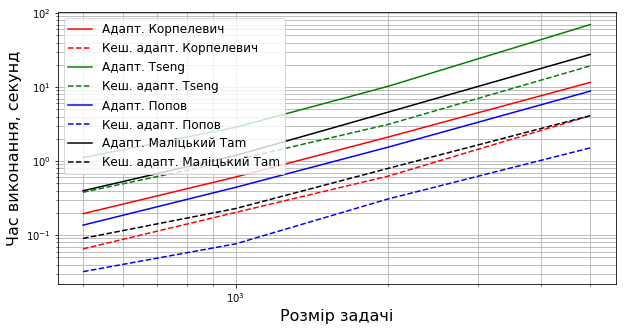
\includegraphics[width=.75\textwidth]{img/4/adapt/time.png}
\end{figure}

Та сама інформація у табличці:

\begin{table}[H]
	\centering
	\begin{tabular}{|c||c|c|c|c|}\hline
		Розмір задачі & 500 & 1000 & 2000 & 5000 \\ \hline \hline
		Адапт. Корпелевич & 0.19 & 0.61 & 2.12 & 11.56 \\ \hline
		Кеш. адапт. Корпелевич & 0.07 & 0.20 & 0.63 & 4.10 \\ \hline
		Адапт. Tseng & 1.11 & 2.86 & 10.27 & 69.95 \\ \hline
		Кеш. адапт. Tseng & 0.38 & 1.04 & 3.14 & 19.33 \\ \hline
		Адапт. Попов & 0.14 & 0.44 & 1.55 & 8.82 \\ \hline
		Кеш. адапт. Попов & 0.03 & 0.08 & 0.31 & 1.51 \\ \hline
		Адапт. Маліцький Tam & 0.40 & 1.19 & 4.60 & 27.66 \\ \hline
		Кеш. адапт. Маліцький Tam & 0.09 & 0.23 & 0.80 & 4.11 \\ \hline
	\end{tabular}
	\caption{Число ітерацій}
\end{table}


\begin{remark}
    Наша реалізація приблизно у 100 разів швидша за результати наведені у статті \href{https://arxiv.org/abs/1502.04968v1}{[Yura Malitsky, 2015]}. 
\end{remark}

\begin{table}[H]
	\centering
	\begin{tabular}{|c||c|c|c|c|}\hline
		Розмір задачі & 500 & 1000 & 2000 & 5000 \\ \hline \hline
		Адапт. Корпелевич & 111 & 113 & 116 & 119 \\ \hline
		Адапт. Tseng & 558 & 572 & 587 & 605 \\ \hline
		Адапт. Попов & 87 & 89 & 91 & 94 \\ \hline
	\end{tabular}
	\caption{Число ітерацій}
\end{table}


\section{Розріджені матриці}

\begin{figure}[H]
    \centering
    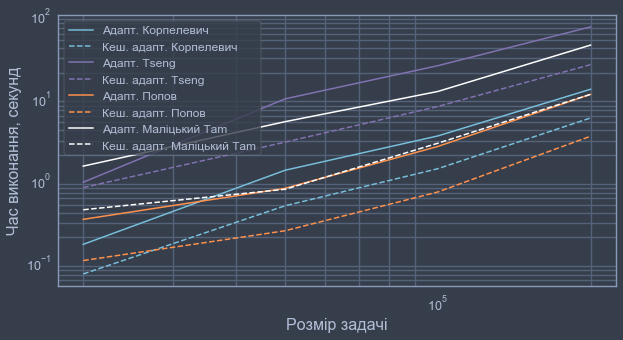
\includegraphics[width=.75\textwidth]{img/4/sparse/adapt/time.png}
\end{figure}

Та сама інформація у табличці:

\begin{table}[H]
	\centering
	\begin{tabular}{|c||c|c|c|c|}\hline
		Розмір задачі & 20000 & 50000 & 100000 & 200000 \\ \hline \hline
		Адапт. Корпелевич & 0.14 & 1.14 & 1.88 & 8.93 \\ \hline
		Кеш. адапт. Корпелевич & 0.07 & 0.45 & 0.96 & 3.87 \\ \hline
		Адапт. Tseng & 1.19 & 4.66 & 10.80 & 54.18 \\ \hline
		Кеш. адапт. Tseng & 0.75 & 1.73 & 3.76 & 19.40 \\ \hline
		Адапт. Попов & 0.34 & 0.59 & 2.39 & 7.84 \\ \hline
		Кеш. адапт. Попов & 0.11 & 0.13 & 0.57 & 2.75 \\ \hline
	\end{tabular}
	\caption{Час виконання, секунд}
\end{table}


\begin{table}[H]
	\centering
	\begin{tabular}{|c||c|c|c|c|}\hline
		Розмір задачі & 20000 & 50000 & 100000 & 200000 \\ \hline \hline
		Адапт. Корпелевич & 74 & 76 & 77 & 79 \\ \hline
		Адапт. Tseng & 388 & 399 & 408 & 416 \\ \hline
		Адапт. Попов & 71 & 73 & 74 & 76 \\ \hline
	\end{tabular}
	\caption{Число ітерацій}
\end{table}


\begin{remark}
    Чомусь на цій задачі алгоритм Tseng'а явно просідає. Причини цього явища поки що не з'ясовані.
\end{remark}
